


This section introduces the company and its activities \Cref{AboutVFT}, the topic of clearing, and the need for risk measures is explained together with its relation to dependency modeling \Cref{Background}. An introduction to copulas is given \Cref{IntroToCopula}. Finally, it motivates this project and specifies its purpose \Cref{Purpose}. 



\subsection{About Vermiculus Financial Technology} \label{AboutVFT}
Vermiculus Financial Technology is a software company that builds systems for financial transactions. Its three main areas of operations are trading systems, clearing systems, and \gls{CSD} systems. Trading systems match buy and sell orders in the market and find the price at which trades should be executed. Clearing systems reduce counterparty risk in financial transactions by acting as the central hub through which all transactions flow. \gls{CSD} systems keep track of who owns which stocks on an exchange.  

This project will be related to the clearing section of Vermiculus activities. 


\subsection{Background}\label{Background}
Clearing systems are in place to minimize counterparty risk in financial transactions\footnote{See \url{https://www.riksbank.se/en-gb/financial-stability/the-financial-system/the-financial-infrastructure/systems-in-the-financial-infrastructure/}. Last Accessed: 2025-01-29}. Counterparty risk is the risk of having the other party in a transaction not fulfilling its obligations in a deal and hence defaulting on its obligations\footnote{See \url{https://www.occ.treas.gov/topics/supervision-and-examination/capital-markets/financial-markets/counterparty-risk/index-counterparty-risk.html}. Last Accessed: 2025-01-29}. 
The clearing house acts as a middleman in all transactions, selling to all buyers and buying to all sellers\footnote{See \url{https://www.investopedia.com/terms/c/clearinghouse.asp}}. Hence, each party only faces the clearing house as their counterparty, removing the counterparty risk, this has been nicely illustrated\footnote{See \url{https://analystprep.com/study-notes/frm/part-1/financial-markets-and-products/central-clearing/}. Last Accessed: 2025-01-29}. In the right part of Figure~\ref{fig:CCP} we can see the clearing members marked B, usually banks, that only face the clearing house marked CCP. In this system, as long as the clearing house does not go bankrupt, trades can go through even if a clearing member defaults on their commitment. The clearinghouse does not offer this risk removal for free; rather, it requires each party to post collateral covering the costs if a clearing member defaults. The clearinghouse makes money from fees and transaction costs, making it worthwhile.

The alternative to centrally cleared trading is that each market participant trades directly with each other. In this case, both sides of a transaction are exposed to counterparty risk from when making a trade until it has been settled. The risk in this scenario is that the buyer does not have enough money to pay or that the seller does not have the asset it has agreed to sell. This is nicely illustrated\footnotemark[\value{footnote}] in the left part of Figure \ref{fig:CCP}. We can see that each clearing member, marked B, faces each other if having the buy and sell side of the same position. In this system, if one of the clearing members defaults, it can impact the other clearing members, who will not get their money. This can cause contagion so if one clearing member goes bankrupt, others may follow suit. 

\begin{figure}[ht]
    \centering
    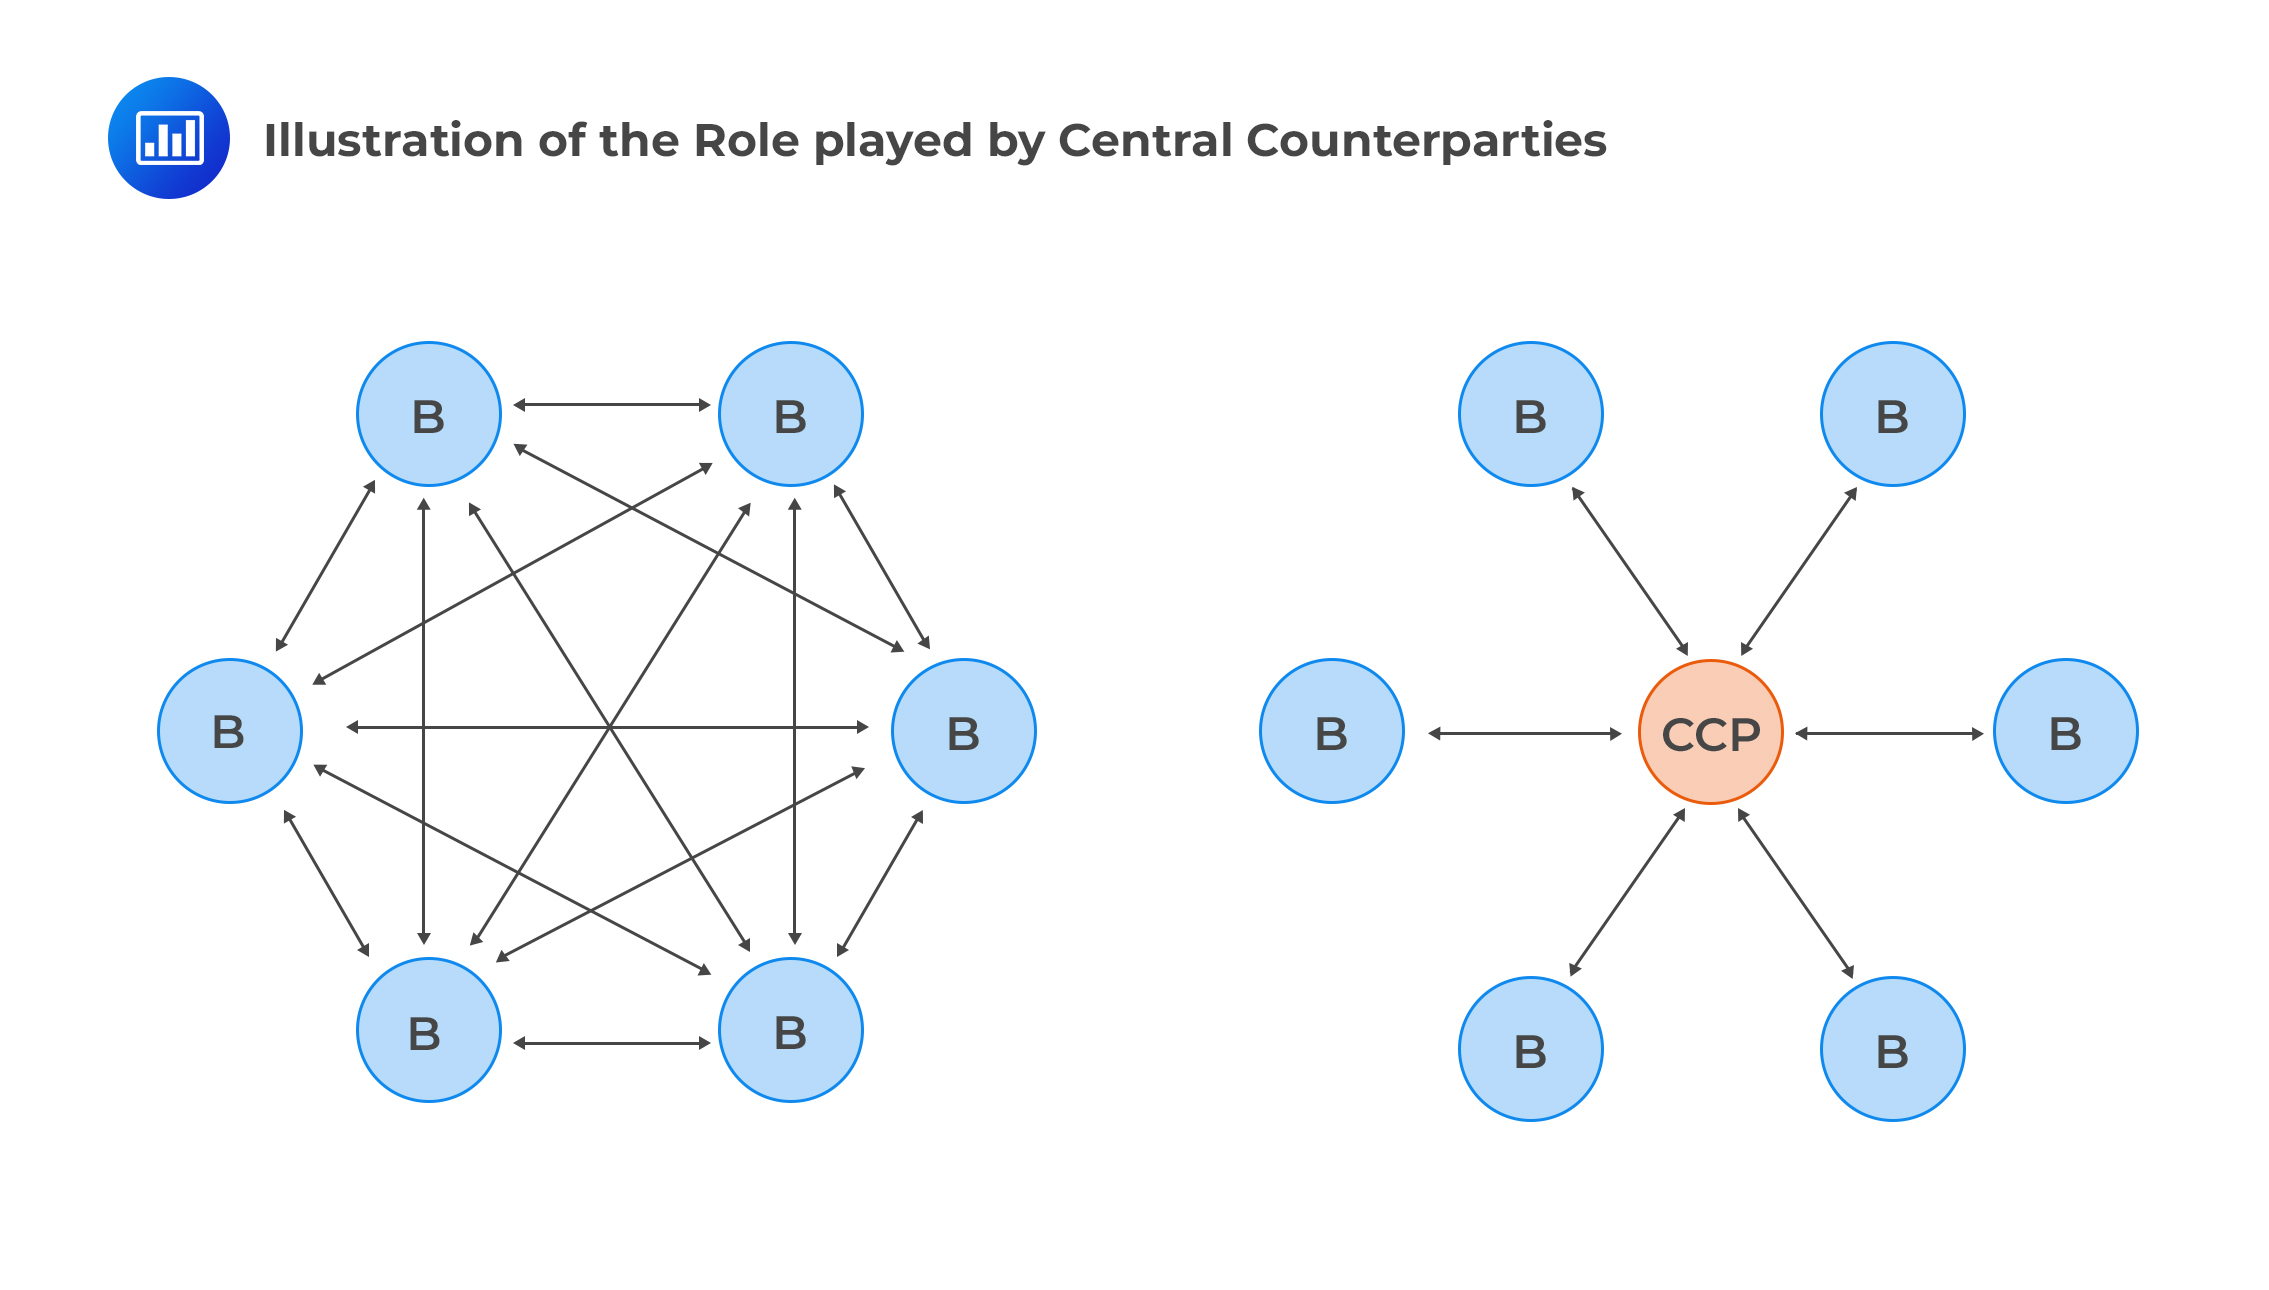
\includegraphics[width=0.7\linewidth]{1Introduction/pictures/CCPvisual .jpg}
    \caption{Bilateral and central counterparty clearing compared. The left picture shows a system of parties that are clearing transactions bilaterally. The right picture shows a system where central counterparty clearing is used. This illustration was found at AnalystPrep\protect\footnotemark[\value{footnote}]. }
    \label{fig:CCP}
\end{figure}

To determine how much collateral is required from each clearing member the risk of its portfolio must be measured. Historically this has been done using a framework called \gls{SPAN} that was developed by Chicago Mercantile Exchange\footnote{See \url{https://www.cmegroup.com/solutions/risk-management/performance-bonds-margins/span-methodology-overview.html\#how-it-works}.  Last Accessed: 2025-01-29}. The \gls{SPAN} framework has several scenarios based on changes in price, volatility, and time to maturity for derivatives. These scenarios are then used to calculate what change in value they would have for some security. Since the global financial crisis in 2008, more focus has been put on risk management. In later years a shift towards using \gls{VaR} has taken place\footnote{See \url{https://www.fia.org/marketvoice/articles/navigating-new-era-derivatives-clearing}}. \gls{VaR} is a measure defined as the maximum expected loss in portfolio value over a time horizon for some level of confidence\footnote{See \url{https://www.risk.net/definition/value-at-risk-var}. Last Accessed: 2025-01-29}. There are several ways of calculating value at risk \gls{VaR} such as historical, parametric, and \gls{MC} simulated among others \footnote{See \url{https://corporatefinanceinstitute.com/resources/career-map/sell-side/risk-management/value-at-risk-var/}}.  

Historical value at risk uses historical returns from the different assets in it to calculate the return of the portfolio at each time step. These portfolio returns are then ordered and the percentile corresponding to the confidence level is calculated giving the \gls{VaR}. This method has advantages and disadvantages. The advantage is that the dependence between assets is completely realistic as it comes from the true observations on the market\footnotemark[\value{footnote}]. A disadvantage is however that this model can be insufficient because the observations from the data are limited. This might sound strange but when observations falling in the tails of a distribution is of course rare. This means that for \gls{VaR}, which focuses on the lower tail, the amount of data available might not be enough to precisely determine the VaR.  

Parametric \gls{VaR} assumes that the returns for an asset are generated from some distribution. These returns are then used for calculating the described characteristics of the distribution. Usually, the Gaussian distribution is used in which case the mean vector and covariance matrix are estimated. This distribution is then used to calculate the \gls{VaR} so that the probability of ending up below the limit aligns with the confidence\footnotemark[\value{footnote}]. This method has the advantage that it is simple. It has a disadvantage in that it requires the data to follow some known distribution which might not always be a realistic assumption.  

\gls{MC} \gls{VaR} utilizes simulated random numbers to generate artificial return scenarios from which the \gls{VaR} can be calculated\footnotemark[\value{footnote}]. \gls{MC} simulations have a major advantage over the other methods mentioned in that they can be used for calculating the risks of different types of financial instruments. This is done by simulating plausible scenarios for the underlying assets of a portfolio.  

The returns need to be simulated from distributions with dependence that reflect how different assets move in relation to one another. There are multiple methods to do this, such as using covariance matrices or copulas. Covariance matrices can be used with different correlation measures such as Pearson, Spearman, and Kendal. Spearman and Kendal are both rank correlation measures, \citet[pp.~256-258]{Alexander2008}. In addition, there are also different types of copulas to use, meaning that there are many alternative methods to choose from. This leads us to the purpose of this project, but first, copulas need to be defined.\todo{Remove about correlation measures }

\subsection{literature review}

\subsection{historical overview }
\begin{generalinstructions}
    On how it links to mathematical finance (credit risk and basket options), what did neural copula do?
\end{generalinstructions}

 
\subsection{Purpose}\label{Purpose}
The purpose of this project is to investigate different methods of modeling dependence and to provide clarity about which method to use for what type of data. While doing this, it is reasonable to expect that shortcomings and risks of different methods will be discovered. In that case, potential shortcomings and risks will be reported to provide an understanding of when different methods can be used. 

\todo{contribution, what is done here and what do I intend to be my contribution}

\textbf{Problem, what is goal
when use copula and neural copula and correlation}
\todo{Specify more}


\subsection{Assignment description}
This thesis will investigate how different methods of modeling dependence between different assets perform for different types of dependency structures. It will also investigate how machine learning can be used as a substitute or complement to better model dependence. 

We will first fit a \gls{NN} as a copula function that captures the dependence between different random variables. The idea is that the copula function can be used for generating new random numbers, with a similar dependency structure to what is observed in the market.   

The following questions will be studied in this project:

%% Aim/Research Questions
\paragraph*{Aim of the thesis.}
\begin{compactenum}[{\bfseries RQ}1]
    \item \label{item:RQ1} Is the marginal distribution used in the \gls{NC} adequate to use?
    \item \label{item:RQ2} How should the neural copula function be trained to obtain consistently reliable results?
    \item \label{item:RQ3} Can a neural copula be used to better model the dependence between asset returns than other copulas?
    
\end{compactenum}
\newcommand{\RQone}{{\bfseries RQ}\ref{item:RQ1}}
\newcommand{\RQtwo}{{\bfseries RQ}\ref{item:RQ2}}
\newcommand{\RQthree}{{\bfseries RQ}\ref{item:RQ3}}
\todo{Change these}


\subsection{Limitations}
To define the scope of this project some limitations will be set initially. In some areas, the constraints are best defined after or during the literature study when more knowledge is obtained. The limitations 


\begin{compactenum}
    \item A selection of traditional measures to compare the \gls{NC} to will be made. 

    \item The number of portfolios will be limited by only considering portfolios with two assets. This will both serve for interpretability and limit the number of portfolios to evaluate. 

    \item The data used will be artificially simulated to control the dependence between the assets in the portfolios and to be able to evaluate each method under consistent conditions. 

    \item The main focus of this report is to implement and evaluate the \gls{NC}. When this is done, other measures will be considered. 
    
\end{compactenum}

These are the initial limitations set for the project. More limitations might be added and the ones defined here might be adjusted.  \todo{change these} 










\textbf{outline of the rest of thesis} 